
% ================================================
\section{Motivation}\label{sec:motication}

Modern Natural Language Processing (NLP) approaches are able to achieve significant results in standard textual analysis tasks. 
The list of tasks includes but is not limited to such fields as text classification, e.g. determining the general topic of the news article \cite{text-classification-Altinel2018} or determining text author's attitude towards the topic \cite{sentiment-analysis-Medhat2014}; sequence tagging,  e.g. named entity recognition (NER)  \cite{ner-Strakova2019,ner-Zhanming2019,ner-Yamada2020,ner-Luoma2020} and part-of-speech tagging \cite{pos-tagging-Bohnet2018}; and text generation \cite{text-gen-Guo2017}. For some applications it is important to combine these tasks to achieve more comprehensible results. 
For instance, in the general case of the sentiment analysis task one aims to classify  whether the author of the piece of text refers to the topic in a negative or positive sense. However, to obtain a finer understanding of why their attitude is inferred to be some particular value, it is important to discern contextual dependencies within the piece, especially in cases when the range of output values goes beyond “polarity” (positive/neutral/negative) and matures into a broader spectrum of values like doubt, contempt, or enjoyment. 
The NLP research community not only actively develops models for improved natural language understanding, i.e. representing language in a vector space, \cite{gpt-Radford2018,bert-Devlin2019,xlnet-Yang2020} but also proposes different fine-tuning approaches for these models \cite{robarta-Liu2019,cr-Joshi2019,gpt2-Radford2019,gpt3-Brown2020}. 

In this project, we aim to perform research in the construction of better textual dependencies for the task in the form of improved Coreference Resolution (CR). 
The CR task is very complex to solve. From 2019 to this date \cite{cr-Joshi2019} no improvement was achieved on the standard benchmark \cite{ontonotes5-Weischedel2013}. 
The recent article \cite{cr-Toshniwal2020} achieved the same metrics as the one from 2019. 
The CR task is a top-level task for contextual understanding in terms of complexity. Nonetheless, the output F1 score of the state-of-the-art approaches shows 79.6\%, which is not sufficient for real-world applications. Hence, the range of possibilities for new solutions is far enough from both exhausting and reaching the saturation point of the research.
 
Coreference resolution combines detection and linking various mentions of entities within the text: linking noun phrases with their counterparts and pronouns, anaphora disambiguation, linking words with their pro-forms, etc.  
Hence, CR-solving models have a significant impact on the quality of the text mining algorithms. 
A good use case where coreference resolution can be applied is categorization of entities and their pronouns to provide one with a broader spectrum of information for future decision making. Based on the extracted data, it is possible to unify all knowledge in the form of a Knowledge Graph (KG) \cite{kg-Wang2017} which can be further utilized for linking concepts represented by textual spans. 
Dependencies and connections between the entities can enrich the feature space with highly discriminative samples for further tasks. 
For example, assume that we have the following two consecutive sentences: “John Smith and Amanda Brown are accountants in XYZ company. Amanda’s colleague was accused of drunk driving”. Based on these sentences, one would wish to classify if some of the entities from the text can be charged for a misdemeanor. 
For a human reader, it is obvious that Amandas’s colleague refers to John. However, for a machine, that is a challenging task. Therefore, proper identification of entity clusters like {John Smith, Amanda’s colleague}, {Amanda Brown}, {XYZ} would significantly improve the machine’s understanding of the piece of text.
Another potential application of coreference resolution lies within the problem of opinion mining in media resources where people frequently freely express their views and opinions.
For example, heated discussions may emerge under political news articles. In these discussions, participants refer to subjects of the particular article with, for instance, pronouns. Therefore, proper CR may provide better traction of the audience's attitude towards entities from the article by linking comment mentions to them.  


In the scope of this work, we expect to improve the current state of the art (see the following section) by means of its further augmentation. 
Firstly, we believe that advancement can be achieved via the modification of the existing CR-solving model which is applied on top of vector embeddings. 
Since the model relies on scoring entity mentions and clustering them, significant changes can be brought with nonlinear dimensionality reduction, which in neural-network-based structures, can be achieved utilizing autoencoders \cite{autoencoders-Zabalza2016,autoencoders-Sahay2019}, since they may enable the model to extract meaningful de-noised relationships from the high-dimensional structure. 
In addition to that, initial tests show that advancements from the named entity recognition field may also provide us with meaningful results, as NER models also focus on entities and context surrounding them: in this case we propose to explore conditional random fields (CRF) \cite{ner-Strakova2019,ner-Zhanming2019,ner-Zhanming2019} and attention \cite{ner-Yamada2020} as potential candidates, as CRF is capable of improving relationship-decoding capabilities of the model and attention learns to put stress on important parts of textual sequences. 
As a further branch of research, we wish to entertain the integration of models uncertainty measurement algorithms e.g deep ensembles \cite{lakshminarayanan2016simple}, MC Dropout \cite{gal2017deep}, SGLD \cite{welling2011bayesian} or Vadam \cite{khan2018fast} to the coreference resolution superstructure for the empirical model weights distribution estimate. The additional information, given the destribution of predicted labels allows faster model learning (hot and warm start methods) with a lower number of training data, given the model prediction uncertainty \cite{sahan2021active}. The architecture agnostic generalization of the empirical model weights distribution estimate will grant us more freedom in the choice of CR task superstructure model with preservation of the precise insight into the model processes given prediction-based uncertainty.
The model uncertainty measurement and its representation is done through the empirical estimate and sampling from the model weights distribution. 
The uncertainty representation approach provides the model with the expanded vision of both model learning and inference. 
The described technique has shown that such algorithms may enhance the learning process significantly \cite{ovadia2019can}.


As another output of this project, we expect to not only push the boundaries of the state-of-the-art algorithms but also create a new Czech and introduce the first Slovak Coreference Resolution datasets generated in an active-learning-powered environment.
Based on the new data and better Coreference Resolution approach, we would like to generalize the CR algorithm as a multilingual solution.


% ================================================
\section{State of the Art}\label{sec:sota}

Modern Coreference Resolution (CR) algorithms are combinations of sophisticated vector embeddings representing context and deep neural network superstructures that perform the coreference resolution itself. 

Natural language understanding (NLU) models. 
The set of existing models for NLU is vast. 
Arguably, one of the most prominent points in history of such models is when the continuous bag-of-words and skip-gram approaches were introduced \cite{w2v-Mikolov2013}. 
At that point machines started to be able to learn the context surrounding particular words and their vector representations  acquired the ability to represent this context, meaning proximity of such vectors in terms of a metric of choice (L2, cosine/angular similarity) veritably described similarity of words or contexts. 
Still, models of these types were far from perfect, as they provided one with constant vectors per word for a pre-set vocabulary. 
Context-dependent representations with flexible vocabularies became available thanks to the introduction of the Transformer architecture \cite{transformer-Vaswani2017} applied on the vocabulary formed not only by words but also by character n-grams constructed as meaningful parts of words.  
The power of the Transformer architecture lies in its encoding and decoding capability improved by the self-attention mechanism which learns to put stress on parts of text sequences. 
This gave birth to a lot of transformer-based language models such as the Bidirectional Encoder Representations from Transformers (BERT) \cite{bert-Devlin2019}, its fine-tuned variations \cite{albert-Lan2020,robarta-Liu2019} and further models \cite{gpt-Radford2018,use-Cer2018}. 
To this date, SpanBERT \cite{cr-Joshi2019} has proven to be one of the most efficient architecture for coreference resolution. 
Its crucial difference from the standard BERT model is that it learns to predict the content of masked spans of text, taking into account their beginnings and endings, omitting the ability of the base BERT model to predict foregoing  sentences, whereas BERT learns to predict the following sentence for each preceding one and attempts to infer individual masked tokens.
Another model worthy of mention is a Longformer whose architecture is based on transformers capable of processing long documents up to 4096 tokens~\cite{Beltagy2020Longformer}.

The first end-to-end coreference resolution model was introduced in \cite{cr-Lee17}. Its crucial difference from its predecessors was that it did not require preprocessing in the form of syntactic parsing or rule-based mention detection, since the model is able to learn mention dependencies on its own to a forerunner-outperforming extent. 
The main idea of the model is to learn to score pairs of textual spans in such a way that takes into account, firstly, if these spans are entity mentions and, secondly, whether the pair is of type antecedent-descendant in terms of coreference.
Span representations are provided by the NLU model of choice. 
The goal is to be able to assign to each span an antecedent span. 
Among the state-of-the-art approaches is \cite{cr-Joshi2019} which utilizes the same structure on top of SpanBERT. 
One of the crucial drawbacks of the scoring approach is the choice of spans: sizes of relevant spans can be different so a constant width of the window may not always be the right choice; spans can either overlap or be disjoint; if they overlap, the value of how large the overlap is also becomes a hyperparameter. 
In addition to that, the number of scoring procedures is quadratic in complexity: each span has to be scored against every its counterpart. 
If the length of the document is large, the memory needed to store all entity mentions may become an issue (in \cite{cr-Xia2020} authors propose an incremental structure for the CR model which needs a lot less memory for the price of a slight decrease in performance).
While previous models are able to achieve decent results, their memory footprint is significant. 
The authors of~\cite{Kirstain2021S2E} bypassed the need to create span representations, relying on a combination of bilinear functions applied on endpoint token representations. 
In addition to that, the new model is built on top of a Longformer encoder capable of processing long documents. 

The CR scoring model takes as input sequences of high-dimensional word-vectors which were produced by multiple consecutive nonlinear mappings. For that reason, one can assume the resulting language-representing structure is highly nonlinear and noisy. 
In such cases, nonlinear dimensionality reduction helps to preserve crucial information, e.g. probability distribution \cite{dr-VanderMaaten2014} or structure of neighborhood-based local metric spaces \cite{dr-McInnes2018}, while reducing the dimension and noisiness of the space. 
Therefore, by learning vector representations with more informative dimensions with, for example, such neural structures as autoencoders \cite{autoencoders-Zabalza2016,autoencoders-Sahay2019} can lead to improved cluster mention classification results. 
In addition to that, the sequential nature of text and the need to classify relations between entity mentions puts CR close to the field of NER where, for instance, CRF \cite{ner-Strakova2019,ner-Zhanming2019} and attention \cite{ner-Yamada2020,translation-Bahdanau2014} have proven to be good additions  to the sequence-labeling model in the endeavor to learn correct token labels, which is a problem with combinatorial complexity: CRF is capable of decoding of sequential relationships into meaningful labels, which in case of CR may represent relationships between mention spans, whereas attention is able to lay emphasis on trigger words or spans that are essential for the task of question.

Another way to improve the model performance from a different aspect is the addition of the uncertainty measurement. 
The grand research from Google \cite{ovadia2019can} shows that the point-wise estimate of model parameters does not usually result in an optimal approach. 
The models uncertainty measurement through the estimate of the empirical model weights distribution has already shown great results in the active learning fields both in Computer Vision \cite{gal2017deep} and NLP in such tasks like NER \cite{shen2017deep, lowell2018practical}, text classification \cite{an2018deep} and other applications. 
Thus, the model parameters estimated based on uncertainty algorithms: i) deep ensembles \cite{lakshminarayanan2016simple} consisting of $N$ networks trained in parallel from different initial conditions; ii) MC Dropout \cite{gal2017deep} which is an extension of the ordinary dropout that samples binary mask multiplying output of a layer, hence stopping propagation through all neurons where zeros is sampled through the network, the extension applies the sampled mask even for predictions generating samples from the predictive distribution; iii) Stochastic Gradient with Langevin Dynamics (SGLD) \cite{welling2011bayesian} which adds additional noise to the gradient in stochastic gradient descent, will bring more efficient training and predictions. 
Back in 2017, the deep ensembles approach for a CR problem \cite{cr-Lee17} showed a significant increase (3\% F1) in the output metrics which confirms the veracity of the concept.

We aim to utilize the knowledge of these aforementioned fields and adapt it to the CR problem to improve the existing framework.

%{\color{red}
For languages other than English, the state of the art for the CR is arguably even farther behind. 
For example, coreference resolution for Czech was attempted on the PCEDT dataset \cite{pcedt-Hajic2012} in \cite{cr-cz-Novak17}; however, the overall performance of the approach does not reach the mark of 0.7 in terms of F-score. 
In addition to that, no transformer-based NLU model was available at the time. 
We aim to address this in our research, as SpanBERT and Longformers demonstrate superior performance to other neural supervised techniques.
%}

% ================================================
\section{Work Packages}\label{sec:wp}

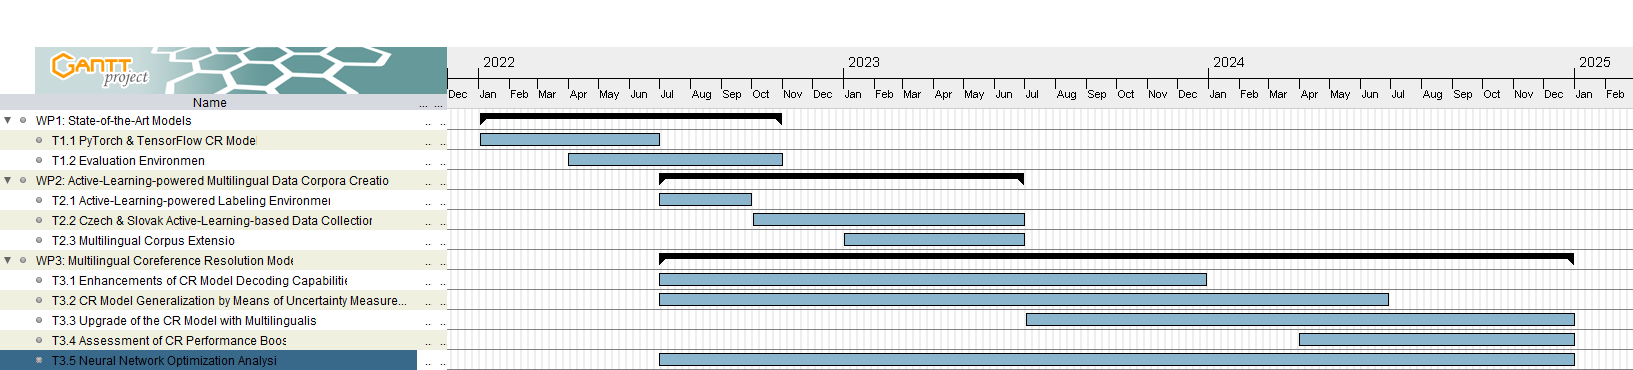
\includegraphics[width=0.99\textwidth]{./figs/Timeschedule}

\subsection*{WP1: State-of-the-Art Models Optimization and Fine-tuning}

%\subsubsection*{T1.1 TBD}
%
%Further enhancement of the state-of-the-art models in PyTorch (\textit{Marko Sahan}) and TensorFlow 2 (\textit{Vladislav Belov}) to support cluster computation optimization and generalization for various text representation mechanisms.
%
%
%\subsubsection*{T1.2 TBD}
%
%Creation of an environment which is capable of assessing and analyzing the quality of the resulting models in a meaningful and comparable way. (\textit{Vladislav Belov, Marko Sahan})


\begin{description}
	\item [T1.1 Enhanced State-of-the-Art CR Models (Belov, Sahan)] Further enhancement of the state-of-the-art models in PyTorch to support cluster computation optimization and generalization for various text representation mechanisms. The existing available implementations are not flexible for experimentation. They are focused on a specific architecture with specific encoding models; some even utilize the Static-Computational-Graph approach. However, modern technologies, e.g., PyTorch and TensorFlow 2, employ Dynamic Computational Graphs \cite{computationalgraph-Neubig2017}. 
	\item [T1.2 Evaluation Environment (Belov, Sahan)] The task of coreference resolution is complex and its performance is evaluated with numerous metrics \cite{muc-Vilain1995,b3-Bagga1998,ceaf-Luo2005}, as the standardly used F1 score \cite{f1-Chen2006} does not embrace all aspects of the discriminative power of features. Therefore, creation of an environment which is capable of assessing and analyzing the quality of the resulting models in a meaningful and comparable way is crucial. The initial structure of the platform is already arranged together with a functioning prototype of~\cite{Kirstain2021S2E}. 
\end{description}


\subsection*{WP2: Active-Learning-powered Multilingual Data Corpora Creation}

 The number of datasets used for benchmarks of coreference-resolution models is quite limited. 
 The most well known one is OntoNotes 5 \cite{ontonotes5-Weischedel2013} and it is only available in English, Chinese and Arabic languages.
 The recently published multilingual harmonized corpus for Czech and ten other languages \cite{cr-mult-Nedoluzhko2021} extends the limits for new models in terms of multilingualism. 
 However, the objective of our research is the creation of the new Active-Learning-Boosted Czech and Slovak datasets optimized for Machine Learning purposes, especially benchmarks on our neural models. 
 The benefit of this package is not only in the development of the new corpus but also in the application of active learning techniques which will reduce the amount of effort annotators put into their work and improve the quality of the resulting data. 

We would like to introduce the Active Learning data corpora creation. The experiment is based on the “smart” way of the data collection when the uncertainty based algorithm will choose the unlabeled data by itself and transfer the instances to the annotators for obtaining the labels. 

\begin{description}
	\item [T2.1 Active-Learning-powered Labeling Environment (Belov, Sahan)] Prepare the active learning data collection and labeling environment.
Modern approach of the data collection is based on the random selection of the documents that may meet some criteria like duplicates removal, etc.. The data for the Czech and Slovak corpus are going to be extracted from online news media and Czech wiki servers. Recent approaches showed that it is possible to select the data batches iteratively with the help of the uncertainty based model feedback both for smaller size batches \cite{gal2017deep, lowell2018practical} and significantly big batches \cite{citovsky2021batch}. The following approach brings the higher quality data selection that also results in less labeling iterations and lower financial expenses.

	\item [T2.2 Czech \& Slovak Active-Learning-based Data Collection (Belov, Sahan)] Creation of Czech and Slovak Data Corpora. The annotations are going to run in the prepared environment from the previous task. In order to reduce the amount of human efforts we will bootstrap the data for the annotations. The bootstrapping approach is based on pre-labeling the Czech and Slovak data with the usage of existing superstructure CR model that uses language independent embeddings for Czech and Slovak language encodings. Described approach will let the annotators to get on average, only task relevant data.
In the first iteration, the target estimate is to have at least 30k-50k annotated sentences for the Czech language. In the second iteration Slovak language data corpus will be collected. The target estimate regarding the annotations is the same as for Czech language (30k-50k). Marko Sahan has the experience of partially leading the end to end 20k sentences corporate corpus creation with entity-to-entity information link labels.  

	\item [T2.3 Multilingual Corpus Extension (Belov, Sahan)] Modern algorithms have a clear traction towards the language-independent approaches like LASER \cite{artetxe2019massively}. 
Thus, the generalization of a coreference task is obvious. Language-independent embeddings approach is a representation of the same semantic structures with the same, or at least similar (with respect to a specific metric) vectors. 
Hence, models trained in English must be able to work with different languages. 
However, in practice, if the model is not fine-tuned with another language that it makes predictions for, the error rate of the predicted instances will be higher (this is the reason for T2.1). 
Nevertheless, modern state of the art approaches were not tested or evaluated on the multilingual datasets either due to the lack of the quality data or due to the fact that the neural CR field is relatively young. 
In addition to CorefUD \cite{cr-mult-Nedoluzhko2021}, we expect to extend our T2.2 data in the same active-learning-enabled environment with 2K-large corpora for French, German, Spanish and Turkish for validation purposes.

\end{description}


\subsection*{WP3: Multilingual Coreference Resolution Model}

WP3 T3.3 and T3.4  are strongly dependent on WP1 and WP2. However WP3 T3.1 can be done in parallel with the WP2 annotation procedure.

\begin{description}
	\item [T3.1 Enhancements of CR Model Decoding Capabilities (Belov)] Investigation of influence of (nonlinear) dimensionality reduction on mention clusters in an attempt to reduce the number of noisy dimensions and improve shapes of these clusters. We will experiment with autoencoders \cite{autoencoders-Zabalza2016,autoencoders-Sahay2019} to achieve a nonlinear mapping of the language-representing manifold onto a lower-dimensional de-noised space within a neural-network model. Moreover, since the models for named entity recognition (NER) also work with entity mentions, examination of superstructures designed for NER, e.g. Conditional Random Fields (CRF) \cite{ner-Strakova2019,ner-Zhanming2019} and entity-aware attention \cite{ner-Yamada2020}, applied on the coreference resolution problem will be further explored.

	\item [T3.2 CR Model Generalization by Means of Uncertainty Measurement (Sahan)] Integration of the uncertainty representations algorithms e.g deep ensembles \cite{lakshminarayanan2016simple}, MC Dropout \cite{gal2017deep}, SGLD \cite{welling2011bayesian} or Vadam \cite{khan2018fast} to the coreference resolution superstructure for the empirical model weights distribution estimate. The beforehand mentioned integration will result in more efficient learning and inference procedures. The primary investigation is concentrated around faster model learning (hot and warm start methods) with a lower number of training data, given the model prediction uncertainty \cite{sahan2021active}. The diversity of embedding-based superstructure model architectures makes the models' uncertainty prediction slow and inefficient. The further step in the uncertainty estimate research is a generalization of the uncertainty given different models architectures (e.g. Vadam \cite{khan2018fast}). The output of the study will allow us to use the architecture agnostic empirical model weights distribution estimate for better noise measurement, faster learning, and label distribution prediction, specifically for different types of CR task embedding superstructure.

	\item [T3.3 Upgrade of the CR Model with Multilingualism (Belov, Sahan)] Generalization to multilingual CR superstructure via usage of multilingual NLU models will allow us to evaluate (retrain and test) the CR superstructure from WP1 on the data from WP2 both for base state-of-the-art models and improved models with potentially a more efficient architecture and the uncertainty representation algorithms. The environment prepared in WP1 will enable us to retrain and to get the results consistently and in faster timelines. 


	\item  [T3.4 Assessment of CR Performance Boost (Belov, Sahan)]  Assessment of influence produced by approaches proposed in T3.1 and T3.2 by means of systematic measurement of relevant metrics \cite{muc-Vilain1995,b3-Bagga1998,ceaf-Luo2005}. Detailed evaluation of contribution provided by each of the proposed solutions both on the currently existing benchmark for English, Arabic, and Chinese \cite{ontonotes5-Weischedel2013} and on the newly created Czech \& Slovak corpora. Moreover, in the scope of the validation process, we aim to test multilingual capabilities of the CR approach on the data obtained from T.2.3 which were not accessible to the model during training iterations.
	
	\item [T3.5 Neural Network Optimization Analysis  (Marik)] Approaches based on neural networks deliver excellent results if their architecture is designed adequately for the solved problem. However, if their architecture does not provide solid gradient paths for optimization convergence, it is not easy to discover its deficiencies causing poor performance. To avoid such events in the project, we will create a monitoring tool and suitable visualizations that should help resolve the issues. To tackle a massive amount of optimized neural network parameters, we will utilize sparse representations such as complex networks.

\end{description}


% ================================================
\section{Research Team}\label{sec:research_team}

The research team consists of a senior researcher leading two Ph.D. students. All three have been working in artificial intelligence research for several years, in the last three years focusing on natural language processing methods. Therefore, the design of the objectives of this project is based on the experience gained in the immensely successful publications and bachelor's, project, or diploma theses of both students. Their work has been directly linked to the methods further developed in the proposal of this project. However, the conditions and the need to address coreference resolution also flow from several projects supported by the GAČR and TAČR agencies, which were led or participated in their solution by their supervisor Radek Mařík.

Applicant Radek Mařík was a co-applicant of the GACR GA16-07210S project successfully solved with an excellent evaluation. He has been the team member of several successfully solved projects supported by MSM (LTT18007) and MV0 (VI20152020008, VG20102015053 in the last five years). He is currently the team member of three TAČR projects (TL02000288, FW01010468, TL04000176), of which all are focused on the processing of Czech texts in the field of media news. In project TACR TL02000288, the applicant addresses the issue of clustering of text fragments, clustering metrics, and the possibility of using community detection from complex networks analysis in clustering, which are used as partial steps in the tasks of generating text messages based on structured data, generating summaries, fact-checking, detection and analysis of the significance of events in the news. In many cases, these tasks encounter the issue of resolution co-referencing, the current state of which, either from a theoretical or practical point of view, does not provide a satisfactory performance and prevents obtaining results with much higher resolution.

The team benefits from Radek Mařík's experience gained during his previous 14 years-long industrially AI-oriented research work at Rockwell Automation and CA Technologies, for example resulting in a patent~\cite{Marik2011}. Theory, methods, and properties related to this project have been studied and implemented in more than nine diploma thesis projects, four bachelor theses, dozens of peer-reviewed, WOS / Scopus indexed conferences, and IF journal papers published the last five years. Additional methods and their properties that have been studied during several research projects dealing with different application domains, including for example ProtoSpy focused on monitoring, communication structure reconstruction, safety assessment, and synchronous event detection for network traffic~\cite{Marik2015b,Marik2014a} and might create additional views on coreference resolution issues.

\begin{description}
	\item [The applicant, Ing. Radek Mařík, CSc.,]  is a specialist in complex network analysis combined with machine learning and data mining, used to develop AI techniques, both theoretical and practical, specialized and applied in non-traditional domains (telecommunications, media news, optical sensors, Egyptology, ceramic tile industry). Based on a shared abstract mathematical and algorithmic foundation, the techniques can also be reused in this project. For example, we have already developed methods for consistency maintenance of input data~\cite{Marik2016c}, automated grouping people into families handling uncertainty and logic, automated family tree building, layout, and visualization (various possibilities of visualization, that might be reused in this project for deep neural network internal properties analysis, were implemented in~\cite{Marik2016,Marik2016b,Marik2017d,Marik2017,Marik2018a,Marik2019a}, automated detection of families with a significant level of nepotism using techniques of social network analysis and data mining~\cite{Dulikova2015,Dulikova2017b}, detection of strategic titles and powerful officials using information theory, that has also been successfully tested in media news topic aspect detection related to this project work~\cite{Marik2018c}, reconstruction of administration development during the Old Kingdom using hidden Markov models~\cite{Dulikova2017b,Marik2017e}, specialized methods for community detection in hierarchical multipartite networks capable of uncover coreference relations~\cite{Marik2018d,Belov2020,Zikmund2020}. 
	
Radek Mařík will manage the project. He supervises both Ph.D. students. He will also be responsible for evaluation neural network representation efficiency and their visualizations with the support of complex network analysis methods. Thus, he will deliver feedback on possible improvements to both students.

\item [Ing. Marko Sahan,] a Ph.D. candidate, has focused on active learning for text classification with enhanced uncertainty representation in his diploma thesis~\cite{Sahan2020}. The significant contribution of his work has resulted in the best student paper at the ECNLPIR 2021 conference~\cite{sahan2021active}. He will explore mainly coreference resolution improvements using advanced uncertainty representations.

\item [Ing. Vladislav Belov,] a Ph.D. candidate, has studied Manifold Learning, Relation Mining, and Kernel Density Estimation~\cite{Belov2020}. His work resulted in contributions to CIIS 2021~\cite{Belov2021ML} and ACAI2021~\cite{Belov2021KDE}. He will focus on the influence of nonlinear dimensionality reduction and structural relations (CRF, entity-aware attention) to coreference resolution.

\end{description}

The team operates with sufficient software library implementations covering both processing and visualizations and hardware and software resources sufficient to perform planned simulations, data mining, and advanced neural network-based processing. The planned acquisition of new hardware components will make the research even more efficient. The new invested notebook will enable the analysis of powerful techniques of state-of-art deep learning to detect deficiencies with sufficient visualization support, and it will serve as a baseline processing facility. However, we will also rely on the current hardware and laboratory equipment available at the CTU. Insufficient processing resources might be considered as the risk of the project proposal. Of course, all team members have skills in programming and new rapid method design and implementation, and volume data processing. Diploma thesis students will also implement extensions, improvements, and new algorithms covering required processing.

\section{Benefits and Outputs of the Projects}

We expect to define new methods for solving coreference resolution with better performance applicable to texts in English and supporting Czech. We believe that the outlined strategy using uncertainty representation, representation of structural entities, and nonlinear dimensionality reduction will significantly enhance the performance of CR.
The second output will be to verify the applicability of the proposed techniques in the environment of processing media reports and contributions with emphasis on the Czech environment. Successful deployment would pave the way for a much better, more accurate assessment of the content of media channels and open up the possibility of a more objective assessment of their impact on the public based on processing a massive stream of online messages by tracing coreference of entities.

We expect to deliver a conference paper each year (conferences dedicated to NLP such as CoNLL, ICML, ICDM). However, the main focus will be given to three impact factor journal papers delivered in the second and third years (e.g., Journal of Information Retrieval, Journal of Machine Learning).
